\chapter{Method Validation} \label{chap:validation} \minitoc

\section{Datasets}

% 01: 
    % ref: N(10,2) for 5M
    % target: N(10,2) for 2.5M and U(100,200) after for 2.5M

% 02:
% 03:
% 04:
% 05:
% 06:

We generated multiple synthetic datasets before moving on to real data. Furthermore, we first performed single feature analysis before moving to a multi-feature scenario. The problem of multiple testing (Section \ref{sec:multi-test}) only arises in the latter case so we only apply the Holm-Bonferroni correction (Section \ref{sec:holmbonferroni}) for that one.

\subsection{Synthetic datasets}
For each test we generated two datasets: one to be used by our method as the reference period and the other as the target or streaming period.

\subsubsection*{Reference and Target Datasets 01}
The Reference Dataset 01 (RD01) contained 5 million events each with a single feature \emph{x1} that followed a normal distribution with mean $\mu=10$ and $\sigma=2$. The Target Dataset 01 (TD01) was also made up of 5 million events each with a single feature. For the first half of the dataset, \textit{i.e.}, for the first 2.5 million events, similarly to the reference dataset, the feature followed a normal distribution with mean $\mu=10$ and $\sigma=2$. However, for the other half, the last 2.5 million events, we changed the generating distribution to be a continuous uniform one with $a=100$ and $b=200$.

\begin{minipage}{.5\textwidth}
  \centering
  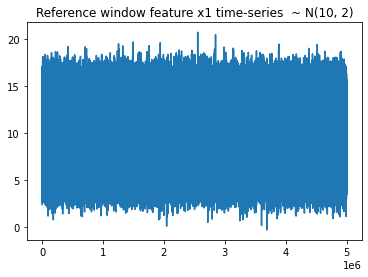
\includegraphics[width=.9\linewidth]{figures/01-reference.png}
  \captionof{figure}{Reference dataset 01 (RD01)}
  \label{fig:rd01}
\end{minipage}%
\begin{minipage}{.5\textwidth}
  \centering
  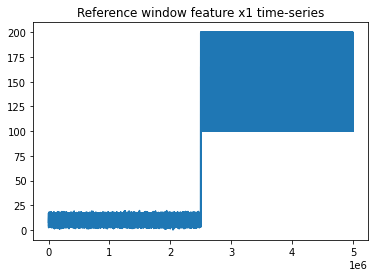
\includegraphics[width=.9\linewidth]{figures/01-target.png}
  \captionof{figure}{Target dataset 01 (TD01)}
  \label{fig:td01}
\end{minipage}


\subsection{Financial fraud datasets}

\section{Experimental Setup}
\subsection{Single feature}
\subsection{Multi feature}

\section{Results}
\subsection{Single feature}
\subsection{Multi feature}

\section{Conclusions}
